% -*- mode: LaTeX; mode: TeX-PDF; coding: utf-8  -*-

\label{sec:func_recv}

\subsection*{Алгоритм восстановления данных}

Восстановление значения в произвольном  узле $x$    мелкой сетки %в узле $x$,
$r$ раз непрерывно дифференцируемой функции $\varphi$
выполняется следующим образом: 
\begin{gather}
  \label{eq:recv_common}
  G_h(\varphi, x) = \sum_{k\in  \Delta_{K,r}}
   \varphi(u^{(k)})
   \psi_{h, r+\mathbf{2}^n}(x-u^{(k)}),%\\ \notag \text{где}\ 
 \end{gather}
 где $ \Delta_{K,r}=\left[-\lfloor{(r+1)/2}\rfloor:
   K-\mathbf{1}^n+\lfloor{(r+1)/2}\rfloor\right]$.  %\cap\mathbb{Z}_+^n

% <!? а тут тоже надо $\mathbf{1}^n)$ и  $\mathbf{2}^n$ !?>

Из формулы~\eqref{eq:recv_common} следует, что для вычислений
могут быть нужны дополнительные
узлы по краям исходной сетки.
Способы выбора значений в этих узлах зависят
от специфики задачи для которой применяется формула~\eqref{eq:recv_common}  
и в данной работе не рассматриваются.


%%%%%%%%%%%%%%%%%%%%%%%%%%%%%%%%%%%%%%%%%%%%%%%%%%%%%%%%%%%%%%%%%
\subsection*{Схема вычислений}


Введём  следующие обозначения.
\begin{itemize}

\item
  $F$  --- массив  известных значений функции $\varphi$
  в узлах крупной сетки;

\item
  $G_r$ --- массив
  значений аппроксимирующей функции в узлах мелкой сетки,
  вычисленных по формуле~\eqref{eq:recv_common};

\item
  $\Psi_{\rho}$ --- массив  значений ядер В. А. Стеклова порядка $\rho$.

\end{itemize}

%Учитывая финитность и симметрию ядер В. А. Стеклова
%в массиве $\Psi_{2}$ нужно хранить $N^*$
%значений ядер $\psi_{2}$;
%%на одном интервале крупной сетки;
%в массиве $\Psi_{4}$ нужно хранить $2N^*$
%значений ядер $\psi_{4}$.
%на двух смежных интервалах крупной сетки.

Учитывая финитность и симметрию ядер В. А. Стеклова
в массиве $\Psi_{r}$ достаточно хранить $\overline{N(r/\mathbf{2}^n + \mathbf{1}^n) +\mathbf{1}^n}$
значений.

% \emph{Сюда можно вставить рисунок 2D ядра 2го порядка для наглядности.
% Выделить ту четвертинку, которую храним.}
Пример ядра порядка 4 на рисунке, $N=4$.

\begin{figure}[h!]
  \centering
  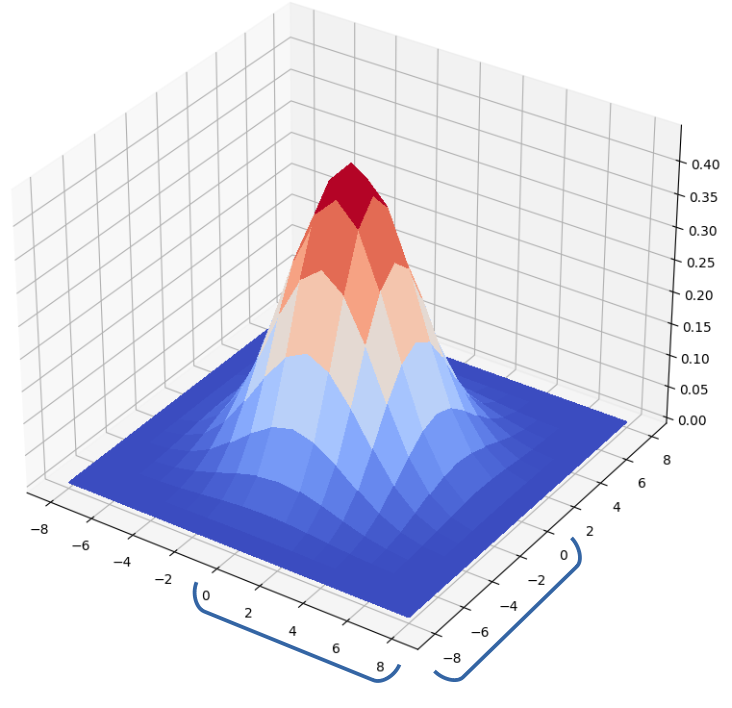
\includegraphics[width=\textwidth
   % ,height
  ]{kern_4_4} 
  \caption{Ядро 4го порядка}
  \label{fig:reg_net}
\end{figure}
\FloatBarrier




Далее приведены выражения для формирования
элементов искомых значений в узлах мелкой сетки,
где $n$ -- количество координат (размерность задачи).

%\emph{Итоговая формула, м.б. от массивов вернуться к функциям?}

\begin{equation}
  \label{eq:nd}
  \begin{split}
    G_r[m] &= 
    \sum_{i \in  [\mathbf{0}^n:r/\mathbf{2}^n + \mathbf{1}^n]} 
        F \left[ \left \lfloor {m}/{N} \right \rfloor - i\right]
      \Psi_{r+\mathbf{2}^n}[iN + m\bmod N] 
       + \\
    &  +
      F \left[\left\lfloor m/N \right \rfloor + (i+\mathbf{1}^n)  \right]
      \Psi_{r+\mathbf{2}^n}[(i+\mathbf{1}^n)N - m \bmod N]
  \end{split}
\end{equation}

На вычисления по формуле~\eqref{eq:nd} требуется

в двумерном случае (2 - операции * и +, 4 части)

$2 * 4 * \overline{(r/\mathbf{2}^n+\mathbf{1}^n) M}.$

в общем случае (2 - операции * и +, $2^n$ частей)

$2 * 2^n * \overline{(r/\mathbf{2}^n+\mathbf{1}^n) M}.$

арифметических операций.

%+(n-1) сложений --- потому что надо сложить результаты по координатам
%А именно для вычисления на одну точку мелкой сетки по каждой координате (2*((r_j+2)-1)) операций:
%(r_j+2) умножение
%и на одно сложение меньше

%По одной координате выражение имеет вид:
% Если $A$ --- $n$-мерный массив, то $[A[i_j]]_j$ означает срез по $j$-й координате, т.~е.
% $A[i_1,\ldots,i_{j-1},i_j,i_{j+1},\ldots,j_n]$, где $i_l$ фиксированы при $l\neq j$.

% \begin{equation}
%   \label{eq:1d}
%   \begin{split}
%     [G_r[m_j]]_{j} &= 
%     \sum_{i = 0}^{r_j/2 +1}
%     \left[
%         F \left[ \left \lfloor {m_j}/{N_j^*} \right \rfloor - i\right]
%     \right]_{j}
%     \left[
%       \Psi_{r+\mathbf{2}^n}[iN_j^* + m_j\bmod N_j^*] 
%     \right]_{j}
%        + \\
%     &  +
%     \left[
%       F \left[\left\lfloor {m_j}/{N_j^*} \right \rfloor + (i+1) \right]
%     \right]_{j}
%     \left[
%       \Psi_{r+\mathbf{2}^n}[(i+1)N_j^* - m_j \bmod N_j^*]
%     \right]_{j}
%   \end{split}
% \end{equation}

\begin{comment}
\emph{Двумерный случай:}

\begin{equation*}
  \begin{split}
    G_r[m_1,m_2] &= 
    \sum_{i_1 = 0}^{r_1/2 +1} \sum_{i_2 = 0}^{r_2/2 +1}
        F \left[ \left \lfloor {m_1}/{N_1} \right \rfloor - i_1, \left \lfloor {m_2}/{N_2} \right \rfloor - i_2\right]
      \Psi_{r_1+2,r_2+2}[i_1N_1 + m_1\bmod N_1,i_2N_2 + m_2\bmod N_2] 
       + \\
    &  +
      F \left[\left\lfloor {m_1}/{N_1} \right \rfloor + (i_1+1), \left\lfloor {m_2}/{N_2} \right \rfloor + (i_2+1)  \right]
      \Psi_{r_1+2,r_2+2}[(i_1+1)N_1 - m_1 \bmod N_1,(i_2+1)N_2 - m_2 \bmod N_2]
  \end{split}
\end{equation*}
  
\end{comment}


Иллюстрация при $r=2$ суммирования по одной координате на рисунке.
\begin{figure}[h!]
  \centering
  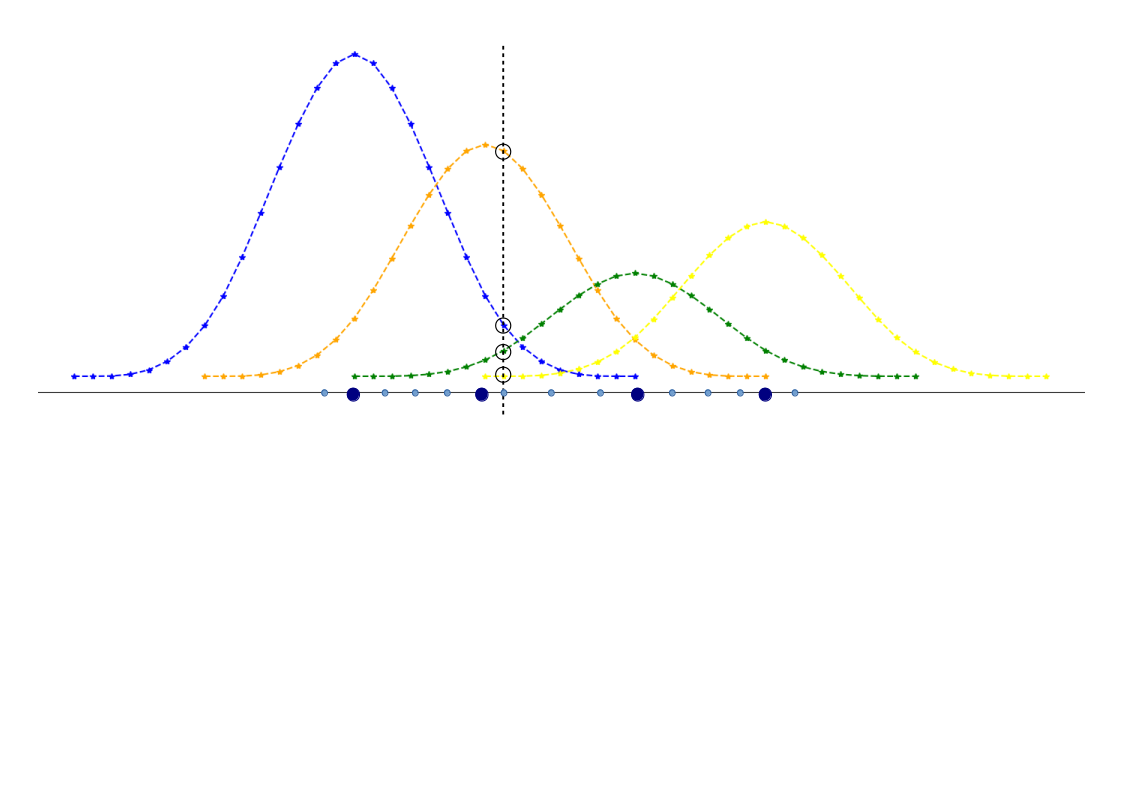
\includegraphics[width=\textwidth,
  %  height=7cm
  ]{multi_kern} 
  \caption{пример для одной координаты}
  \label{fig:reg_net}
\end{figure}
\FloatBarrier



% Заметка про этапы индексации.
% \emph{Можно как=то учесть в обозначениях}
% \begin{enumerate}
% \item
%   Лоцировать ячейку в которой находится искомая точка мелкой сетки.
%   Операция $\left \lfloor \frac{m_j}{N_j^*} \right \rfloor$.

% \item
%   Отобразить индекс в координатах всей мелкой сетки на координаты в ячейке.
%   Операция $m_j \bmod N_j^*$.
% \end{enumerate}
  


%%
\begin{comment}
\begin{itemize}

  \item
Для восстановления данных без сглаживания искомые 
значения в узлах мелкой сетки формируются следующим образом: 
\begin{equation}
  \label{eq:recv_r0}
  \begin{split}
  G_0(m) &=
  F \left( \left \lfloor \frac{m}{N} \right \rfloor \right)\Psi_{2}(m\bmod N) +{}\\
 &+ F \left( \left \lfloor \frac{m}{N} \right \rfloor + 1 \right)\Psi_{2}(N - m \bmod N),
  \end{split}
\end{equation}
где $m = 0, \ldots, M-1$.

Количество арифметических операций при вычислениях непосредственно по формуле~\eqref{eq:recv_r0}
равно $3M$.
%Вычисления по формуле~\eqref{eq:recv_r0} далее будем обозначать алгоритм А1.

\item
%А при $r = 2$ формула~\eqref{eq:recv_common} 
%представляется следующим образом.
Выражение для восстановления данных со сглаживанием имеет вид:
\begin{equation}
  \label{eq:recv_r2}
\begin{split}
  G_2(m) &=  F \left(\left \lfloor \frac{m}{N} \right \rfloor - 1 \right)
              \Psi_{4}(N + m \bmod N)   + {}\\
              &+ F \left (\left \lfloor \frac{m}{N} \right \rfloor \right)
              \Psi_{4}(m \bmod N) +{}\\
              &+ F \left( \left \lfloor \frac{m}{N} \right \rfloor
              + 1 \right)\Psi_{4}(N - m \bmod N)  + {}\\
              &+ F \left(\left \lfloor \frac{m}{N} \right \rfloor + 2 \right)
              \Psi_{4}(2N - m \bmod N),
\end{split}
\end{equation}
где $m = 0, \ldots, M-1$.

Количество арифметических операций при вычислениях непосредственно по формуле~\eqref{eq:recv_r2}
равно $7M$.
%Вычисления по формуле~\eqref{eq:recv_r2} далее будем обозначать алгоритм А2.

\end{itemize}
\end{comment}


Заметим, 
что в формуле~\eqref{eq:nd} каждое из произведений известного значения в узле крупной сетки
со значениями ядер в узлах мелкой сетки используется несколько раз
при формировании результатов в нескольких соседних
%интервалах
ячейках 
крупной сетки. 
С учётом этого факта,
предложена следующая двухэтапная вычислительная схема.
\begin{enumerate}
\item
  %Вычисление произведений значений ядер в узлах мелкой сетки
  %для каждого узла крупной сетки.
  Вычисление для $k$-го ($k \in [0:K-\mathbf{1}^n]$)
  известного значения функции 
  элементов массива произведений
  $\Pi_r[k,l] = F[k]\Psi_{r+\mathbf{2}^n}[l]$,
  ($l \in [0:r(N-\mathbf{1}^n)/2]$).

  Выполняется $\overline{K (N(r/\mathbf{2}^n + \mathbf{1}^n) +\mathbf{1}^n)}$ умножений.
  %$\prod_{i=1}^n K_i(r_iN_i)/2^n$ 
  

\item
  Выбор и суммирование полученных на предыдущем шаге произведений
  для формирования результирующих значений в узлах мелкой сетки
  следующим образом 
\begin{equation}
  \label{eq:nd}
  \begin{split}
    G_r[m] &= 
    \sum_{i \in  [\mathbf{0}^n:r/\mathbf{2}^n + \mathbf{1}^n]} 
        \Pi_r \left[ \left \lfloor {m}/{N} \right \rfloor - i\right, iN + m\bmod N] 
       + \\
    &  +
      \Pi_r\left[\left\lfloor m/N \right \rfloor + (i+\mathbf{1}^n)  \right, (i+\mathbf{1}^n)N - m \bmod N]. 
  \end{split}
\end{equation}

%\emph {в общем случае (2 - операции * и +, 2^n частей) }
%$2 * 2^n * \overline{(r/2+1) M}.$

  Выполняется $2^n * \overline{(r^n/\mathbf{2}^n+\mathbf{1}^n) M}$ сложений.


  %Выполняется $r^2M$ сложений.
  %$M$ сложений в первом варианте и
  %$3M$ сложений --- во втором.
\end{enumerate}

Всего на вычисления по данной схеме требуется

$\overline{K (N(r/\mathbf{2}^n + \mathbf{1}^n) +\mathbf{1}^n)} + 2^n * \overline{(r/\mathbf{2}^n+\mathbf{1}^n) M}$
арифметических операций
вместо

$2^n * \overline{(r/2+\mathbf{1}^n) M} + 2^n * \overline{(r/2+\mathbf{1}^n) M}.$

т.е. сложений одинаковое количество, а умножений

$\overline{K (N(r/\mathbf{2}^n + \mathbf{1}^n) +\mathbf{1}^n)}$

что должно оказаться меньше, чем $2^n * \overline{(r/2+\mathbf{1}^n) M}$.

По порядку значений $KN = M$, тогда выигрыш (примерно) в $2^n$ раз в умножениях. 

%При такой схеме вычислений общее количество арифметических операций
%для восстановления данных без сглаживания
%составляет $2KN + 2K - N$ (что меньше, чем $3M = 3NK + 3K - 3N$)
%и $5KN + 5K - 3N$ (что меньше, чем $7M = 7NK + 7K - 7N$) для
%восстановления данных со сглаживанием.

%Задача восстановления данных в узлах мелкой сетки
%рассматривается как одна стадия конвейера в модели БСКП.
%ВПД этой стадии является массив $F$ размером $K$,
%содержащий известные
%значения в узлах крупной сетки.
%Обработка ВПД  %восстановления значений в узлах мелкой сетки
%состоит из двух вычислительных процедур,
%соответствующих перечисленным выше этапам.


Иллюстрация вычислительной схемы на рисунке.
\begin{figure}[h!]
  \centering
  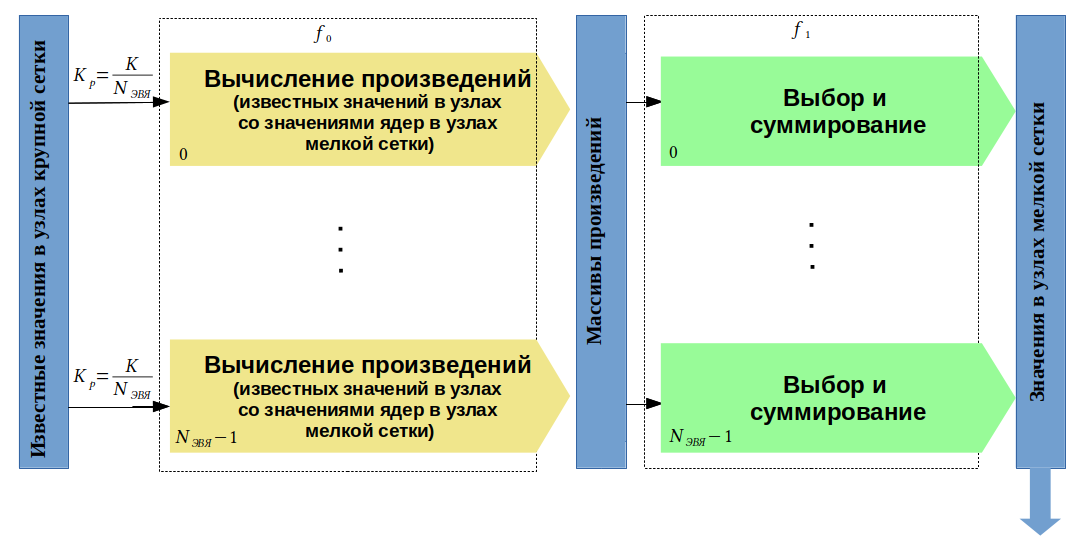
\includegraphics[width=\textwidth,height=7cm]{comp_scheme_steps} 
  \caption{Двухэтапная вычислительная схема}
  \label{fig:reg_net}
\end{figure}
\FloatBarrier


%%%%%%%%%%%%
%-->
%%%%%%%%%%%
\begin{comment}
\subsection*{Параллельные алгоритмы}
Алгоритмы восстановления данных без сглаживания и со сглаживанием
обладают параллелизмом по данным. 
Пусть данная стадия выполняется на ВВЭ состоящем из  $P$ ЭЦСП.
%Значения в узлах крупной сетки
%распределены между всеми ЭЦСП равномерно и размещены в их глобальной памяти.

Рассмотрим вариант равномерного размещения значений в узлах крупной сетки при условии, что
между вычислительными элементами на обоих уровнях модели БСКП
(т.~е. как между ЭЦСП, так и между ЭВЯ) предполагается обмен данными.
Тогда на $p$-м ЭЦСП ($p = 0, \ldots, P-1$)
обрабатывается $K_p = K/P$ узлов, $K_p < GMem$.
Каждый ЭЦСП 
параллельно с остальными обрабатывает свою часть
крупной сетки из $K_p$ узлов и
формирует часть мелкой сетки размером $M_p = N(K_p-1) + K_p$.
Эти узлы, в свою очередь, 
%распределены,
разбиты 
на ЭПД для вычислений на ЭВЯ.
Размер каждого ЭПД $K_p^j = K_p/N_\text{ЭВЯ}$, где $j = 0, \ldots, N_{\text{ЭВЯ}}-1$.
Здесь, для простоты изложения, считаем, что $K_p^j < {LMem}/{2}$,
$K_p$ кратно $N_{\text{ЭВЯ}}$, а $K$ кратно $P$.
%Если эти условия не выполняются, то потребуется обработка дополнительных ЭПД. 

%При таком размещении исходных узлов 
На втором этапе вычислительной схемы в формировании узлов мелкой сетки
на крайних интервалах каждой из частей крупной сетки  
участвуют произведения, которые оказались вычисленными в соседних
вычислительных элементах. % (ЭЦСП или ЭВЯ).
%Поэтому требуется обмен данными.
В случае восстановления данных без сглаживания
каждый вычислительный элемент должен получить дополнительные $N$ значений,
со сглаживанием --- дополнительные $4N$ значений.

Если обмен данными между вычислительными элементами на каком-либо из уровней модели БСКП
исключается,  
то необходимо дублировать данные в крайних узлах частей крупной сетки в соседних
вычислительных элементах.
Для алгоритма без сглаживания в каждом вычислительном элементе размещается $K_p+1$ узлов 
крупной сетки и вычисляется на $N$ больше произведений,
а для алгоритма со сглаживанием --- по $K_p + 3$ узла
и вычисляется на $4N$ произведений больше.


Предложенный подход к распараллеливанию по данным 
эффективен, если на одном ЭЦСП обрабатывается %(без учёта дублирования)
$K_p \ge 2 N_{\text{ЭВЯ}}$ узлов крупной сетки для алгоритма без сглаживания и
$K_p \ge 4 N_{\text{ЭВЯ}}$ узлов для алгоритма co сглаживанием.
Следовательно, границы масштабируемости параллельных алгоритмов восстановления данных 
определются следующими неравенствами:
$P \le \left \lfloor \frac{K}{2N_{\text{ЭВЯ}}} \right \rfloor$ для алгоритма 
без сглаживания и 
$P \le \left \lfloor \frac{K}{4N_{\text{ЭВЯ}}} \right \rfloor$ для
алгоритма со сглаживанием.
%сетки значительно
%больше количества вычислительных элементов и
%выражается следующим
%соотношении размера крупной сетки и количества вычислительных элементов:
%$K \ge 4P$.

%\emph{Тут Можно кол-во операций в табличке представить!}
В таблице~\ref{tab:common_compl} приведены
выражения вычислительной сложности $W$,
коммуникационной сложности $H$ и
количества барьерных синхронизаций $S$,
необходимых для 
трёх вариантов 
параллельных вычислительных алгоритмов
восстановления значений в узлах мелкой сетки %без сглаживания
по формуле~\eqref{eq:recv_r0} и
%со сглаживанием
по формуле~\eqref{eq:recv_r2}.
%на P вычислительных элементах 

\begin{table}[h!] 
  \begin{tabular}{|p{0.17\textwidth}|p{0.38\textwidth}|p{0.38\textwidth}|}
    %%
    \hline
    & без сглаживания & со сглаживанием \\
    \hline
    Без применения двухэтапной вычислительной схемы  &
    %    $$W = \frac{3(NK + K)}{P} - 3N$$
    $$W = 3K_{p}(N + 1) - 3N$$
    $$H = 0; \ S = 0$$ & 
    %    $$W = \frac{7(NK + K)}{P} - 7N$$
    $$W = 7K_{p}(N + 1) - 7N$$
    $$H = 0; \ S = 0$$ 
    \\
    \hline
    По двухэтапной вычислительной схеме с обменами &
    %    $$W = \frac{2(NK + K)}{P} - N$$
    $$W = 2K_{p}(N + 1) - N$$
    $$H = N+1; \ S = 1$$ & 
    %    $$W = \frac{5(NK + K)}{P} - 3N$$
    $$W = 5K_p(N + 1) - 3N$$
    $$H = 4(N+1); \ S = 1$$ 
    \\
    \hline
    По двухэтапной вычислительной схеме без обменов &
    %    $$W = \frac{2(NK + K)}{P} + 1$$
    $$W = 2K_{p}(N + 1) + 1$$
    $$H = 0; \ S = 1$$ & 
    %    $$W = \frac{5(NK + K)}{P} + 3N + 6$$
    $$W = 5K_{p}(N + 1) + N + 4$$
    $$H = 0; \ S = 1$$ 
    \\
    \hline
  \end{tabular}
  \caption {Сводная таблица со сложностями параллельных алгоритмов
    восстановления значений в узлах мелкой сетки}
  \label{tab:common_compl}
\end{table}
%\FloatBarrier 

Из таблицы~\ref{tab:common_compl} видно, что  
алгоритмы с передачей данных и без передачи данных
имеют одинаковую сложность, если пропускная способность, 
с которой вычислительные элементы могут обмениваться данными, равна единице.
Если эта пропускная способность меньше единицы,
то эффективнее алгоритм с передачей данных, а 
если больше, то выгоднее посчитать лишние произведения и данные не передавать.
%Но выбор между алгоритмом с передачей данных и алгоритмом с дополнительными вычислениями,
%но без передачи в конечном итоге зависит от архитектурных особенностей целевой системы.
%Например, даже при условии низкой пропускной способности коммуникационной среды
%если система поддерживает DMA (т. е. предоставляет возможность передачи данных на фоне вычислений),
%то велика вероятность, что эффективнее окажется вариант алгоритма с передачей данных.
\end{comment}


\begin{comment}
\subsection*{Описание программной реализации}

Алгоритмы восстановления данных без сглаживания и со сглаживанием
реализованы в виде библиотеки функций на языке Си.
%Далее рассматриваются подробно действия на каждом из супершагов
%для алгоритмов восстановлений со сглаживанием и без сглаживания.
%При этом именно такая последовательность супершагов в алгоритме со сглаживанием
%позволяет эффективно использовать память.
Каждый из них состоит из двух вычислительных процедур. 
Рассмотрим подробнее реализованные для этих алгоритмов вычислительные процедуры.

\subsubsection{Алгоритм А1 для восстановления данных в узлах мелкой сетки без сглаживания}
%Параллельный алгоритм для 
%вычисления значений в узлах мелкой сетки
%по формуле~\eqref{eq:recv_r0} (т.~е. без сглаживания)
%в терминах модели BSP состоит из двух <<супершагов>>.

\begin{enumerate}
\item
  Каждый вычислительный элемент выполняет следующие действия.
  
  \begin{itemize}
  \item
    Формирует $N$ элементов массива произведений
    $\Pi_2$  
    для первого узла 
    части крупной сетки, обрабатываемой на текущем вычислительном элементе.
%    со значениями ядер В. А. Стеклова
%    второго порядка (вычислены на этапе инициализации и хранятся в памяти).
    
  \item
    В случае варианта реализации с обменами:  
    посылает $N$ значений сформированных %для крайнего узла крупной сетки
    произведений другому вычислительному элементу
    (где обрабатывается предыдущая часть крупной сетки).
    
  \item
    В случае варианта реализации без обменов:
    вычисляет $N$ элементов массива произведений
    $\Pi_2$  
    для дополнительного $K_p$-го узла
    части крупной сетки при наличии этого узла. 
    Если обрабатываемая часть сетки %последняя ---b
    содержит узел с номером $K-1$, то 
    формируется <<код отсутствия>>.
  \end{itemize}
  
\item
  Каждый вычислительный элемент выполняет следующие действия.

  \begin{itemize}
  \item
    В случае варианта реализации с обменами:
    принимает $N$ дополнительных значений произведений
    (которые необходимы для формирования
    значений в узлах мелкой сетки на крайнем справа интервале)
    или <<код отсутствия>>,
    если обрабатываемая на вычислительном элементе
    часть сетки %является последней.
    содержит узел с номером $K-1$.
  \item
    В случае варианта реализации без обменов:
    в качестве дополнительных значений используются
    произведения для $K_p$-го узла,
    сформированные текущим вычислительным элементом
    в предыдущей вычислительной процедуре. 
    
  \item
    Независимо формирует оставшиеся $(K_p - 1)N$ произведений 
    и вычисляет попарным суммированием соответствующих произведений
    $K_p N$ значение в узлах мелкой сетки
    при наличии дополнительных данных %от другого вычислительного элемента
    или
    $(K_p-1) N$ значений в случае <<кода отсутствия>>.
  \end{itemize}
\end{enumerate}


\subsubsection{Алгоритм А2 для восстановления данных в узлах мелкой сетки со сглаживанием}
%Параллельный алгоритм для 
%вычисления значений в узлах мелкой сетки со сглаживанием 
%по формуле~\eqref{eq:recv_r2} 
%в терминах модели BSP состоит из двух <<супершагов>>.

\begin{enumerate}
  \item
    Каждый вычислительный элемент выполняет следующие действия.
    \begin{itemize}
    \item
      Формирует %$3(2N + 2) $ значений произведений
      три массива произведений $\Pi_4$ для 
      узлов с номерами 0, 1  и $K_p - 1$ части крупной сетки, обрабатываемой на текущем
      вычислительном элементе. 
%      со значениями
%      ядер В.~А.~Стеклова четвёртого порядка.

    \item
      В случае варианта реализации с обменами: 
      посылает
      $2N$ значений произведений для 0-го узла текущей части крупной сетки и  %$K_p - 2$
      $N$ значений произведений для 1-го узла текущей части крупной сетки %$K_p - 1$ и
      вычислительному элементу, где обрабатывается предыдущая часть крупной сетки, 
      а $N$ значений произведений для последнего узла --- 
      вычислительному элементу, где обрабатывается её следующая часть.

    \item
      В случае варианта реализации без обменов:
      вычисляет $N$ элементов массива произведений
      $\Pi_4(n)$, $n = N, \ldots, 2N-1$, для 
      дополнительного узла слева;
      $2N$ элементов массива произведений
      $\Pi_4(n)$, $n = 0, \ldots, 2N-1$,
      для первого дополнительного узла справа;  
      $N$ элементов массива произведений
      $\Pi_4(n)$, $n = N, \ldots, 2N-1$, 
      для второго дополнительного узла справа.
      В случае отсутствия какого-либо из дополнительных узлов
      вместо соответствующих произведений формируются <<коды отсутствия>>. 
    \end{itemize}
    
  \item
    Каждый вычислительный элемент выполняет следующие действия.
    \begin{itemize}
    \item
      В случае варианта реализации с обменами: 
      принимает $4N$ дополнительных 
      значений произведений
      или <<коды отсутствия>>.
      
    \item
      В случае варианта реализации без обменов:
      вместо принятых значений произведений используются
      произведения для соответствующих дополнительных узлов,
      сформированные текущим вычислительным элементом
      в предыдущей вычислительной процедуре. 

    \item
      Независимо формирует $2N(K_p - 3)$
      оставшихся  произведений
      и суммирует по 4 соответствующих произведения, получая
      $K_p N$ значений в узлах мелкой сетки при наличии
      дополнительных данных справа или  
      %от вычислительного элемента, где обрабатывается следующая часть исходной крупной сетки или
      $(K_p-1) N$ значений --- если часть сетки %является последней.
      содержит узел с номером $K-1$.
    \end{itemize}
\end{enumerate}

 
%\emph{Замечание про <<кольцевой буфер>>.} 
Объединение суммирования с формированием произведений для не крайних
узлов крупной сетки во второй вычислительной процедуре  
позволяет сократить объём памяти, необходимой для хранения
значений произведений. Вместо хранения второго экземпляра мелкой сетки
со всеми значениями произведений можно хранить 
$2 \times N$ или
$4 \times 2N$
произведений соответственно, которые нужны для
вычисления значений в узлах мелкой сетки на
текущем интервале.
Для организации хранения произведений применяется структура данных
<<кольцевой буфер>>.

\end{comment}

%%
%\bibitem {Zhuk}
%Жук~В.~В. Методические указания к курсу <<Теория аппроксимации функций и ее
%приложения>>. Часть 2. С.-Петербургский ун-т. 1993. 41~с.


%%% Local Variables: 
%%% mode: latex
%%% TeX-master: "paper_func_recv"
%%% End: 



